\documentclass{IEEEtran} 

%%you can call packages here 
\usepackage[utf8]{inputenc} %utf8 text character encoding
\usepackage{cite}
\usepackage{amsmath,amssymb,amsfonts,nccmath}
\usepackage{hyperref}
\hypersetup{colorlinks,linkcolor={blue},citecolor={blue},urlcolor={red}}  
\usepackage{cleveref} %Para usar crefrange
\usepackage{algorithm,algorithmic}
\usepackage{graphicx}
\usepackage{textcomp}
\usepackage[font=footnotesize,labelfont=bf]{caption}
\usepackage[font=footnotesize,labelfont=bf]{subcaption}
\usepackage{color}
\usepackage{gensymb}
\usepackage{dblfloatfix}
\usepackage{lineno}
\usepackage{enumitem}
\usepackage[autostyle]{csquotes}
\usepackage{latexsym} 


\title{Ensayo sobre IoT y IoE}
\author{Cervantes Contreras Brando} 


\begin{document}
\maketitle

%%\vspace{-13mm}

\section{Introduction} \label{introduction}
 According to an article published in 2015 reference as \cite{chui2010internet}, even though it isnt quite new, it has an interesting approach
 about how the internet of things could be evolving in the near future and how it is perceived.
 It says that, the physical world itself is becoming a type of information system.
 Where everything being connected, objects itself can sense the environment 
 and communicate, they become some sort of tools for understanding 
 the complexity of the modern world and respond to it.
 What’s revolutionary in all this is that these physical information systems are now beginning to 
 be deployed, and some of them even work largely without human intervention.


%%GRAMMARLY 

\section{Objectives}

First we'll give some definitions.
\subsection{Internet of Things (IoT)}
From what I understand, IoT can be defined as the possibility of giving everyday objects the ability to identify themselves, by using sensors and actuators, 
and then communicate with other objects 
through wired and wireless networks, often using the same Internet Protocol (IP). These networks will carry high volumes of data for computers for analysis, and will 
return information that are valuable to us.
Some types of applications for IoT are:
\begin{enumerate}
     \item Consumer Type
     \begin{itemize}
          \item HomeAndOffice -  Some examples are Smart Houses, Programmed Light, Smart consume.
          \item Wearables - IoWt (Internet of wearable things) they are usually small and are part of everyday use, also portable and highly responsive. 
          Smart watches, Elders monitoring and voice control are some.
     \end{itemize}
     \item Commercial Type
     \begin{itemize}
          \item Medical care (quick and more accurate measurement)
          \item Transportation (smart parking)
          \item Construction and home automation (Control of energy consumption)
     \end{itemize}

\end{enumerate}

\subsection{Internet of Everything (IoE)}
IoE is like a IoT but amplified, because it covers a wider connectivity where network intelligence works as the main part. It is the intelligent integration 
and connection between 4 key elements:
\begin{enumerate}
     \item People
     \item Process
     \item Data 
     \item Things 
\end{enumerate}

The main difference between IoT and IoE is that in IoE human intervention is needed, so a higher decision-making and business model also.


\section{Questions }\label{systemModel}
\begin{itemize}
     \item \textbf{What IoT/IoE Projects do you know?}
     
     The majority of IoT projects that i know are pretty simple and the Home-Office type, the ones that 
     you interact with daily, like a smartwatch, a washing machine or a security camera.
     But there's also one that I found recently and came to my attention, it assures to be the first IoT device, it can be referenced as \cite{xu2015animal},
     what i found interesting about it is that it arose based on a common need, it was invented 
     as nothing too serious, beacuse the american campus with the idea just wanted to monitor the expending
     machines and have the colas always cold, in spite of it, they'd decided to use Arpanet network to connect it
     with the rest of the machines and make something that eventually would become too big to handle.

     \item \textbf{What IoT/IoE Projects have used?}
     
     IoE none. But, I've used cameras, washing machines, smartwatch, the TV, and even a car stereo.
     The installation, most of the times is pretty simple and intuitive, but still
     if you want to create a wider network, maybe that's when it gets tricky.

     \item \textbf{What IoT/IoE Projects have you developed?}
     
     None. Even though, in high school i'd developed a rain filtering roof and if i had knew 
     about IoT, i surely would have implemented it on my project.

     \item \textbf{What IoT/IoE Projects do you want to develop?}
     
     I´ve been thinking about this one quite a few months ago, but I don´t take it too much 
     of a deal because it may sound a little silly or probably even a very common one. It is a 
     smart coffee maker that gets turn on according to your alarm clock, so when you are all  
     ready to get out, you can carry your coffe with you, all warm and on time.
     Maybe there´s already one out there with the same specs, but if i could develop my own i would
     add a more sophisticated system and a much better method of filtering and preparing 
     the coffee.
     \begin{figure}
          \centering
          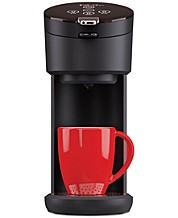
\includegraphics[width=3 cm]{coffeem.jpg}
          \caption{Coffe Maker}
          \label{thermalmonitoring}
     \end{figure}
     

\end{itemize}


\section{Future
projects/technologies}
I think this tecnology it's only starting and will get much wilder and powerful 
eventually, until the human comfort will no longer need to be satisfied, which 
we can guess would be lot of time for it to happen.


\section{Conclusions}

A fascinating world of interconnection of objects, measuring variables, gathering information about the environment, about health, about our homes, and mostly about us.
It is extremely important to develop knowledge in this area together with the idea of the importance of the security of this type of connection, how safe we can make the transmission of our information.

El internet de las cosas es mas que nada el futuro y evolucion del tan avanzado uso de la mayor red a nivel global, el internet, asi mismo el mundo de las comunicaciones
va de la mano con el descubrimiento y acceso a la informacion, esto significa que garantiza que todo esta tecnología seguira en constante evolución hasta un punto en que todo este conectado 
, para que esto se lleve a cabo muy probablemente se encontraran mas formas de medir los datos a traves de sensores y actuadores, cada vez, mas sofisticados y puede ser 
que hasta mas baratos para mayor numero y alcance. Solo me deja pensando que si todo se encuentra conectado, ¿será mas facil para terceros el acceder a nuestra información 
confidencial?, ¿de verdad es buena idea dejar todo en manos de algo que puede en algun punto dado llegar a salirse de nuestro control?. 
(Me parecío importante dar una parte de la conclusion en español para abarcar mayor profundidad y poder explayarme un poco mas.)

\bibliographystyle{ieeetran}


\bibliography{References2}

\end{document}





